\documentclass[12pt,letterpaper]{article}

\usepackage[utf8]{inputenc}
\usepackage[T1]{fontenc}
\usepackage[spanish,es-tabla]{babel}
\usepackage[margin=2.54cm]{geometry}
\usepackage{newtxtext,newtxmath}
\usepackage{microtype}
\usepackage{setspace}
\usepackage{graphicx}
\usepackage{xcolor}
\usepackage{tikz}
\usepackage{booktabs}
\usepackage{array}
\usepackage{tabularx}
\usepackage{caption}
\usepackage{fancyhdr}
\usepackage{titlesec}
\usepackage{enumitem}
\usepackage{float}
\usepackage[hidelinks]{hyperref}

% Paleta inspirada en el Bosque de Niebla y Sendero Vivo 3D
\definecolor{forestDark}{HTML}{164A32}
\definecolor{forestMid}{HTML}{1F6B48}
\definecolor{forestSage}{HTML}{78A88D}
\definecolor{forestMist}{HTML}{E6F0EA}
\definecolor{woodWarm}{HTML}{9E5A22}
\definecolor{inkDark}{HTML}{18241C}
\definecolor{mutedGray}{HTML}{4A5950}

% Configuración de enlaces clicables
\hypersetup{
  colorlinks=true,
  linkcolor=forestDark,
  urlcolor=forestDark,
  citecolor=inkDark,
  pdftitle={Informe Laboratorio 1 - Sendero Vivo 3D},
  pdfauthor={Jordan Guamán, Mesías Mariscal, Denise Rea}
}

% Formato Normas APA 7.ª edición
\setlength{\parindent}{1.27cm}
\setlength{\parskip}{0pt}
\setcounter{secnumdepth}{0}

\titleformat{\section}
  {\normalfont\fontsize{12}{14}\bfseries\centering}
  {}{0pt}{}
\titlespacing*{\section}{0pt}{14pt}{6pt}

\titleformat{\subsection}
  {\normalfont\fontsize{12}{14}\bfseries\raggedright}
  {}{0pt}{}
\titlespacing*{\subsection}{0pt}{12pt}{4pt}

\titleformat{\subsubsection}
  {\normalfont\fontsize{12}{14}\bfseries\itshape\raggedright}
  {}{0pt}{}
\titlespacing*{\subsubsection}{0pt}{10pt}{2pt}

% Encabezado y numeración APA 7 (titulillo izquierda, página derecha)
\pagestyle{fancy}
\fancyhf{}
\fancyhead[L]{\fontsize{9}{11}\selectfont\color{mutedGray}SENDERO VIVO 3D: ECOTURISMO COMUNITARIO ACCESIBLE}
\fancyhead[R]{\fontsize{10}{12}\selectfont\thepage}
\renewcommand{\headrulewidth}{0pt}
\setlength{\headheight}{15pt}

\newcolumntype{L}[1]{>{\raggedright\arraybackslash}p{#1}}
\captionsetup[table]{
  labelsep=newline,
  singlelinecheck=false,
  justification=raggedright,
  labelfont=bf,
  textfont=it,
  skip=4pt
}

\begin{document}

% ============================================================================
% PORTADA MINIMALISTA INSTITUCIONAL ESPE (INSPIRACIÓN TEMÁTICA SUTIL)
% ============================================================================
\begin{titlepage}
\thispagestyle{empty}

% Trazo minimalista lineal al pie (sin rellenos pesados ni tarjetas)
\begin{tikzpicture}[remember picture, overlay]
  % Línea superior muy fina
  \draw[forestDark, line width=1.4pt]
    ([xshift=2.54cm, yshift=-1.65cm]current page.north west)
    -- ([xshift=-2.54cm, yshift=-1.65cm]current page.north east);

  % Silueta lineal minimalista de montaña y sendero al pie de página
  \draw[forestSage!80, line width=0.8pt]
    ([xshift=2.54cm, yshift=1.95cm]current page.south west)
    .. controls ([xshift=6.5cm, yshift=2.55cm]current page.south west)
    and ([xshift=9.2cm, yshift=1.85cm]current page.south west)
    .. ([xshift=12.4cm, yshift=2.45cm]current page.south west)
    .. controls ([xshift=15.0cm, yshift=2.90cm]current page.south west)
    and ([xshift=17.2cm, yshift=2.05cm]current page.south west)
    .. ([xshift=-2.54cm, yshift=2.15cm]current page.south east);

  \draw[woodWarm!75, line width=0.9pt]
    ([xshift=2.54cm, yshift=1.65cm]current page.south west)
    .. controls ([xshift=7.5cm, yshift=2.05cm]current page.south west)
    and ([xshift=13.5cm, yshift=1.45cm]current page.south west)
    .. ([xshift=-2.54cm, yshift=1.85cm]current page.south east);
\end{tikzpicture}

\centering
\vspace*{0.15cm}
{\fontsize{13.5}{16}\selectfont\bfseries\color{inkDark} UNIVERSIDAD DE LAS FUERZAS ARMADAS ESPE\par}
\vspace{0.4cm}


\includegraphics[width=3.2cm]{assets/espe_logo.jpg}\par
\vspace{0.35cm}

{\fontsize{11.5}{14}\selectfont\bfseries\color{inkDark} DEPARTAMENTO DE CIENCIAS DE LA COMUNICACIÓN\par}
\vspace{0.35cm}

{\fontsize{10.5}{13}\selectfont\bfseries CARRERA\par}
{\fontsize{11}{14}\selectfont INGENIERÍA EN SOFTWARE\par}
\vspace{0.25cm}

{\fontsize{10.5}{13}\selectfont\bfseries ASIGNATURA\par}
{\fontsize{11}{14}\selectfont DESARROLLO DE SOFTWARE APLICADO AL DOMINIO DE INTERCULTURALIDAD\par}

\vspace{0.45cm}
% Divisor minimalista con emblema botánico lineal
\begin{tikzpicture}
  \draw[forestSage, line width=0.6pt] (-5.8,0) -- (-0.55,0);
  \draw[forestSage, line width=0.6pt] (0.55,0) -- (5.8,0);
  \draw[forestMid, line width=0.85pt] (0,-0.16) .. controls (0.22,-0.02) and (0.22,0.16) .. (0,0.22)
    .. controls (-0.22,0.16) and (-0.22,-0.02) .. (0,-0.16);
  \draw[forestMid, line width=0.6pt] (0,-0.22) -- (0,0.16);
\end{tikzpicture}\par
\vspace{0.42cm}

{\fontsize{10}{13}\selectfont\bfseries\color{woodWarm} LABORATORIO 1\par}
\vspace{0.18cm}
{\fontsize{14}{18}\selectfont\bfseries\color{forestDark} SENDERO VIVO 3D: ECOTURISMO COMUNITARIO Y NATURALEZA ACCESIBLE\par}
\vspace{0.12cm}
{\fontsize{10.5}{14}\selectfont\itshape\color{mutedGray} Desarrollo de un prototipo de aplicación inmersiva inclusiva y definición de necesidades\par}

\vspace{0.45cm}
{\color{forestSage}\rule{0.72\textwidth}{0.5pt}}\par
\vspace{0.45cm}

{\fontsize{10.5}{13}\selectfont\bfseries INTEGRANTES\par}
\vspace{0.1cm}
{\fontsize{11}{15}\selectfont
Jordan Guamán \\
Mesías Mariscal \\
Denise Rea\par}

\vspace{0.32cm}
{\fontsize{10.5}{13}\selectfont\bfseries DOCENTE\par}
\vspace{0.08cm}
{\fontsize{11}{14}\selectfont ING. ENRIQUE CALVOPIÑA\par}

\vspace{0.32cm}
{\fontsize{10.5}{13}\selectfont\bfseries FECHA\par}
\vspace{0.08cm}
{\fontsize{11}{14}\selectfont 16 de noviembre de 2026\par}

\vspace{0.55cm}
{\color{forestSage}\rule{0.72\textwidth}{0.5pt}}\par
\vspace{0.25cm}
{\fontsize{9.5}{13.5}\selectfont
\textbf{\color{forestDark}Repositorio GitHub:} \url{https://github.com/AMVMesias/sendero-vivo-3d} \\
\textbf{\color{forestDark}Aplicación Web (Vercel):} \url{https://museo-abierto-3d.vercel.app}\par}

\vfill
\end{titlepage}

% ============================================================================
% PÁGINA 2: FICHA DE ACCESO MINIMALISTA Y RESUMEN (APA 7)
% ============================================================================
\setcounter{page}{2}

\noindent\textbf{Ficha de Acceso y Publicación del Prototipo}
\vspace{4pt}

\begingroup
\setstretch{1.2}
\fontsize{10}{13}\selectfont
\noindent\begin{tabularx}{\textwidth}{@{}L{4.2cm} >{\raggedright\arraybackslash}X@{}}
\toprule
\textbf{Repositorio GitHub} & \url{https://github.com/AMVMesias/sendero-vivo-3d} \\
\textbf{Despliegue en vivo (Vercel)} & \url{https://museo-abierto-3d.vercel.app} \\
\textbf{Rama principal} & \texttt{main} \\
\textbf{Tecnologías} & Vite, Three.js, Web Audio API, Web Speech API, HTML5, CSS3 e iconografía SVG propia \\
\textbf{Grupo vulnerable} & Personas con movilidad reducida (silla de ruedas, bastón o andador) y adultos mayores \\
\bottomrule
\end{tabularx}
\endgroup

\vspace{0.45cm}

\doublespacing

\section{Resumen}

\noindent El acceso al ocio, a la naturaleza y al encuentro con las culturas locales suele verse restringido por barreras físicas, geográficas, económicas y sensoriales que afectan de manera desproporcionada a las personas con movilidad reducida y a los adultos mayores. El presente informe documenta los resultados del Laboratorio 1, correspondientes a la selección fundamentada de un grupo vulnerable, la definición de sus necesidades multidimensionales y el desarrollo de \textit{Sendero Vivo 3D}, un prototipo web inmersivo e inclusivo de ecoturismo comunitario accesible. La solución implementa una pasarela virtual continua de 250 metros sin escalones ni pendientes abruptas, distribuida en seis estaciones representativas de un bosque de niebla y guiada por relatos comunitarios. Entre sus mecanismos de accesibilidad destacan la perspectiva ergonómica ajustable entre silla de ruedas (1,15 m) y vista de pie (1,65 m), controles de mirada sin arrastre, avance continuo tramo a tramo, modo de paseo guiado automático, texto escalable, alto contraste, reducción de movimiento, paisaje sonoro procedural y narración en voz alta en español. El prototipo incorpora texturas fotorrealistas e iconografía vectorial propia, y se encuentra publicado en GitHub y desplegado en producción mediante Vercel.

\vspace{0.2cm}
\noindent\textit{Palabras clave:} accesibilidad universal, ecoturismo comunitario, interculturalidad, realidad virtual web, movilidad reducida, adultos mayores.

\newpage

% ============================================================================
% CUERPO DEL INFORME (APA 7)
% ============================================================================
\section{Introducción}

El derecho a la recreación, al disfrute del patrimonio natural y a la participación cultural en igualdad de condiciones constituye un principio básico de equidad social. Sin embargo, gran parte de los destinos de turismo rural, reservas ecológicas y senderos comunitarios en América Latina carecen de infraestructura universal: presentan terrenos irregulares, escalinatas, barro o largas distancias desde las ciudades que excluyen sistemáticamente a las personas con movilidad reducida y a los adultos mayores (Organización Mundial del Turismo [OMT], 2014). En el contexto ecuatoriano, el artículo 44 de la Ley Orgánica de Discapacidades (Asamblea Nacional del Ecuador, 2012) establece el deber de garantizar ofertas de turismo accesible basadas en el diseño universal; no obstante, su implementación física en territorios rurales enfrenta limitaciones presupuestarias y topográficas.

Desde la perspectiva de la interculturalidad crítica, la exclusión territorial no solo impide el esparcimiento individual, sino que también fractura el diálogo horizontal entre habitantes urbanos en situación de vulnerabilidad y comunidades rurales portadoras de saberes ecológicos, medicinales y artesanales (Walsh, 2009). Asimismo, la Organización Mundial de la Salud (OMS, 2022) advierte que alrededor de 1.300 millones de personas en el mundo viven con algún tipo de discapacidad y enfrentan barreras estructurales persistentes que agravan el aislamiento y la inequidad.

En respuesta a esta problemática, el Laboratorio 1 plantea la definición rigurosa de necesidades de un grupo vulnerable específico y la construcción de un prototipo funcional denominado \textit{Sendero Vivo 3D}. A diferencia de los entornos museográficos tradicionales cerrados, la propuesta recrea un ecosistema vivo de bosque de niebla a través de una aplicación web 3D ejecutable en cualquier navegador estándar, demostrando cómo el diseño inclusivo puede acercar territorios rurales inaccesibles mientras visibiliza la economía solidaria local.

\section{Selección y Caracterización del Grupo Vulnerable}

\subsection{Delimitación del Grupo Seleccionado}

Para evitar planteamientos genéricos, se delimitó como grupo vulnerable principal a las \textbf{personas con movilidad reducida} —particularmente usuarios de silla de ruedas, bastón o andador— y a los \textbf{adultos mayores con limitaciones físicas o de desplazamiento prolongado}. Aunque ambos colectivos presentan particularidades propias, comparten un denominador común crítico frente al entorno natural: la imposibilidad o alta dificultad para transitar rutas montañosas sin pavimento, sortear raíces expuestas, cruzar quebradas o costear traslados especializados hacia zonas rurales alejadas.

\subsection{Barreras Físicas, Sensoriales y Socioculturales}

La revisión de principios internacionales de turismo accesible permite identificar la llamada \textit{cadena de accesibilidad}: si un solo eslabón falla (transporte, sendero, señalética o descanso), la experiencia completa resulta inaccesible (OMT, 2014). En el caso del grupo seleccionado concurren cuatro barreras principales:

\begin{enumerate}[leftmargin=2.2cm, itemsep=2pt]
  \item \textbf{Barreras arquitectónicas y topográficas:} ausencia de pasarelas niveladas, pendientes superiores al límite ergonómico, escalones naturales y falta de zonas de descanso intermedias.
  \item \textbf{Barreras sensoriales y de interfaz digital:} muchas aplicaciones 3D exigen visores de realidad virtual costosos o movimientos rápidos de cámara que provocan fatiga motriz y cinetosis (mareo vestibular), además de emplear tipografías diminutas poco legibles para adultos mayores con presbicia.
  \item \textbf{Barreras económicas y tecnológicas:} requerimiento de equipos de cómputo de gama alta o desplazamiento presencial costoso.
  \item \textbf{Aislamiento social y distancia intercultural:} confinamiento domiciliario o urbano que limita el vínculo afectivo con la naturaleza y el conocimiento directo de comunidades rurales anfitrionas.
\end{enumerate}

\section{Definición y Matriz de Necesidades}

A partir de las barreras identificadas y de las pautas internacionales de accesibilidad web WCAG 2.2 (World Wide Web Consortium [W3C], 2023), se estructuraron cinco dimensiones de necesidades que orientaron cada decisión de diseño del prototipo \textit{Sendero Vivo 3D}. La Tabla 1 sintetiza esta matriz de trazabilidad entre las necesidades del usuario y las soluciones implementadas.

\begin{table}[H]
\centering
\caption{Matriz de necesidades multidimensionales del grupo vulnerable y respuestas de diseño}
\label{tab:necesidades}
\setstretch{1.15}
\fontsize{9.5}{12}\selectfont
\begin{tabularx}{\textwidth}{L{2.5cm} L{5.0cm} >{\raggedright\arraybackslash}X}
\toprule
\textbf{Dimensión} & \textbf{Necesidad identificada} & \textbf{Respuesta en \textit{Sendero Vivo 3D}} \\
\midrule
Física y motora &
Recorrer un entorno natural sin depender de destreza motriz fina, arrastre sostenido ni combinaciones complejas de teclado. &
Pasarela 3D continua sin escalones; botones amplios ($\geq$ 46 px); atajos \texttt{1}--\texttt{6} y \texttt{W}/\texttt{S}; controles de mirada lateral sin arrastre y modo Paseo guiado automático. \\
\addlinespace[4pt]
Sensorial y vestibular &
Evitar mareos por giros bruscos de cámara y facilitar la lectura ante presbicia o fatiga visual. &
Transiciones suaves o salto directo al activar Reducir movimiento; escalado de texto (Normal, Grande, Muy grande) y modo Alto contraste. \\
\addlinespace[4pt]
Auditiva y cognitiva &
Comprender relatos culturales en lenguaje claro sin sobrecarga técnica y disponer de apoyo sonoro opcional. &
Redacción bajo criterios de Lectura Fácil, narración en voz alta en español (\textit{Web Speech API}) con pausa y velocidad regulable, y paisaje sonoro natural silenciable. \\
\addlinespace[4pt]
Tecnológica y económica &
Acceder sin adquirir gafas de realidad virtual ni instalar software propietario complejo. &
Aplicación Web 3D ligera ejecutada en navegador estándar sobre PC, portátil o tableta con despliegue público en Vercel. \\
\addlinespace[4pt]
Intercultural y ergonómica &
Valorar saberes comunitarios con dignidad y experimentar la escala espacial real de un usuario sentado. &
Relatos centrados en voces locales (medicina tradicional, agua y textiles) y alternancia entre altura de silla de ruedas (1,15 m) y de pie (1,65 m). \\
\bottomrule
\end{tabularx}
\vspace{4pt}
\par\raggedright\fontsize{9}{11}\selectfont\textit{Nota.} Elaboración propia basada en las pautas WCAG 2.2 (W3C, 2023) y los principios de diseño universal de la OMT (2014).
\end{table}

\section{Enfoque Intercultural y Diálogo de Saberes}

La propuesta asume la interculturalidad más allá de la representación ornamental o folclórica del entorno rural. Siguiendo los planteamientos de Walsh (2009), el diálogo intercultural exige reconocer a las comunidades rurales y pueblos originarios como productores legítimos de conocimiento científico, ecológico y social. En consecuencia, las estaciones del recorrido evitan presentar el bosque como un escenario vacío para consumo turístico pasivo y articulan tres ejes narrativos:

\begin{itemize}[leftmargin=2.2cm, itemsep=2pt]
  \item \textbf{Territorio como sujeto vivo:} el relato inicial concibe la montaña y la neblina como un hogar compartido que demanda reciprocidad y respeto antes de recorrerlo.
  \item \textbf{Diálogo horizontal de saberes:} en la huerta elevada comunitaria, el conocimiento tradicional de plantas como la hierba luisa y el romero dialoga con prácticas agroecológicas actuales y adaptaciones ergonómicas reales (bancales a 80 cm de altura).
  \item \textbf{Justicia hídrica y economía solidaria:} la estación de la quebrada visibiliza las mingas comunitarias para proteger vertientes, mientras la ramada final expone textiles con tintes naturales y oficios locales como fuentes de sustento directo para 18 familias anfitrionas.
\end{itemize}

\section{Diseño y Arquitectura del Prototipo Inmersivo}

\subsection{Arquitectura Tecnológica y Modularidad}

El prototipo fue implementado bajo una arquitectura web modular con Vite como empaquetador y Three.js como motor de renderizado WebGL. El código fuente se organizó en capas independientes para facilitar su mantenimiento: \texttt{src/data/stations.js} centraliza el guion intercultural de las seis estaciones; \texttt{src/scene/shaders.js} define programas y extensiones GLSL personalizados para atmósfera, agua, suelo multizona, corteza musgosa y viento; \texttt{src/scene/trailScene.js} construye el terreno, la pasarela, cinco especies arbóreas, sotobosque florido, texturas y cámara ergonómica; \texttt{src/audio/natureAudio.js} sintetiza de forma procedural la brisa, las aves y el murmullo de la cascada mediante \textit{Web Audio API}; \texttt{src/audio/narrator.js} gestiona la lectura en español mediante \textit{Web Speech API}; y \texttt{src/ui/icons.js} provee la iconografía SVG propia de toda la interfaz.

\subsection{Recorrido de 250 Metros y Estaciones Comunitarias}

Para ofrecer una experiencia genuinamente inmersiva y no limitada a una única vista estática, se trazó una curva \textit{Catmull-Rom} de aproximadamente 250 metros conformada por 320 tablones instanciados de madera, pasamanos continuos y pilares cimentados sobre el terreno montañoso. El usuario puede desplazarse estación por estación o avanzar tramo a tramo con los botones de paso continuo y teclas \texttt{W}/\texttt{S}, visualizando un indicador de distancia en tiempo real (\texttt{0 m -- 250 m}). La Tabla 2 detalla las seis estaciones que integran el recorrido.

\begin{table}[H]
\centering
\caption{Estaciones del recorrido accesible de 250 metros, voces comunitarias y adaptaciones}
\label{tab:estaciones}
\setstretch{1.15}
\fontsize{9.5}{12}\selectfont
\begin{tabularx}{\textwidth}{L{0.7cm} L{3.3cm} L{3.0cm} >{\raggedright\arraybackslash}X}
\toprule
\textbf{N.\textsuperscript{o}} & \textbf{Estación} & \textbf{Guía comunitario} & \textbf{Contenido intercultural y adaptación inclusiva} \\
\midrule
1 & Mirador de la Neblina & Doña Rosa Gualinga & Bienvenida territorial, banca con bahía lateral para silla de ruedas y panel físico con mapa botánico ilustrado. \\
\addlinespace[3pt]
2 & Paso de los Árboles Abuelos & Taita Mateo Chimbo & Árbol centenario con raíces tablares y bromelias rodeado por pasarela curva sin compactar el suelo musgoso. \\
\addlinespace[3pt]
3 & Huerta Elevada de Saberes Medicinales & Don Segundo Morales & Tres bancales elevados a 80 cm libres por debajo para aproximar silla de ruedas; plantas aromáticas y medicina tradicional. \\
\addlinespace[3pt]
4 & Quebrada y Cascada del Agua Viva & María Quintero & Puente nivelado sobre el cauce, caída de agua animada entre rocas basálticas y audio adaptativo según cercanía. \\
\addlinespace[3pt]
5 & Mirador de Aves y Descanso Accesible & Lucía Andrade & Pérgola sombreada de descanso para adultos mayores frente a un árbol florido con aves animadas en vuelo suave. \\
\addlinespace[3pt]
6 & Ramada de Oficios y Economía Solidaria & Taller Textil Sumak & Pabellón iluminado con tapices andinos tejidos, ánforas de cerámica sobre mesa accesible y cierre de comercio justo. \\
\bottomrule
\end{tabularx}
\vspace{4pt}
\par\raggedright\fontsize{9}{11}\selectfont\textit{Nota.} Datos correspondientes a la configuración implementada en \texttt{src/data/stations.js}.
\end{table}

\subsection{Shaders GLSL, Texturas Fotorrealistas e Iconografía Personalizada}

Con el propósito de superar la apariencia geométrica plana y ofrecer realismo inmersivo en todo el bosque nublado, se integraron once texturas continuas almacenadas en \texttt{public/textures/} junto con mapas de relieve (\textit{bump maps}) y texturas procedurales de espuma hídrica, cantos rodados de río y frondas plumosas con recorte alfa. Este repertorio cubre tablones envejecidos, roca basáltica húmeda, tres cortezas arbóreas diferenciadas (corteza oscura de árbol abuelo, aliso plateado y \textit{Polylepis} rojizo), dos follajes de copa (verde esmeralda y oliva dorado) y cuatro coberturas de terreno mezcladas por shader según elevación, pendiente y cercanía al arroyo (humus de bosque, pradera florida, grava de río y roca andina). Adicionalmente, los ocho programas y extensiones GLSL en \texttt{src/scene/shaders.js} animan las nubes FBM en domo celeste sin recortes, bruma de valle, caída curva con espuma en la cascada, cáusticas y reflexión Fresnel en el río, musgo en la base de los troncos y balanceo eólico en copas, arbustos floridos y helechos arborescentes curvados.

Para reforzar la identidad cultural y visual del entorno, se incorporaron dos recursos gráficos diseñados a medida: un mapa ecológico ilustrado colocado en el atril de madera del Mirador inicial (Figura 1) y un tejido geométrico andino aplicado tanto en el camino de mesa como en los tapices colgantes de la Ramada comunitaria (Figura 2). Asimismo, se prescindió por completo de emojis del sistema en toda la interfaz, creando un conjunto propio de iconos vectoriales SVG (\texttt{src/ui/icons.js}) que heredan automáticamente los colores del modo estándar y del modo Alto contraste.

\begin{figure}[htbp]
\raggedright
\textbf{Figura 1}\par
\textit{Mapa botánico ilustrado incorporado en el atril de bienvenida del Mirador de la Neblina}\par
\vspace{6pt}
\centering
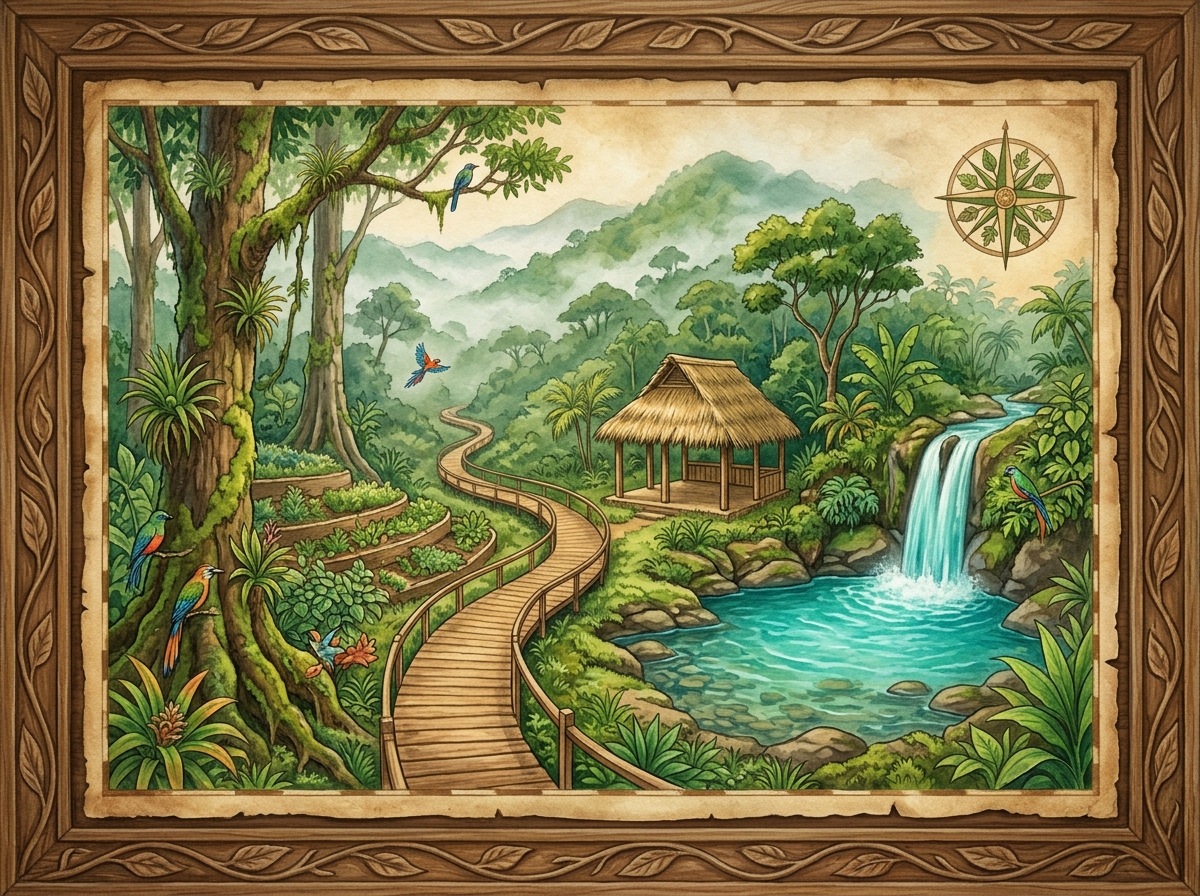
\includegraphics[width=0.65\textwidth]{assets/welcome_map.jpg}\par
\vspace{4pt}
\raggedright\fontsize{9}{11}\selectfont\textit{Nota.} Recurso gráfico ubicado en \texttt{public/textures/welcome\_map.jpg}, renderizado dentro de la Estación 1 como señalética panorámica accesible.
\end{figure}

\begin{figure}[htbp]
\raggedright
\textbf{Figura 2}\par
\textit{Patrón textil artesanal aplicado a los tapices colgantes de la Ramada comunitaria}\par
\vspace{6pt}
\centering
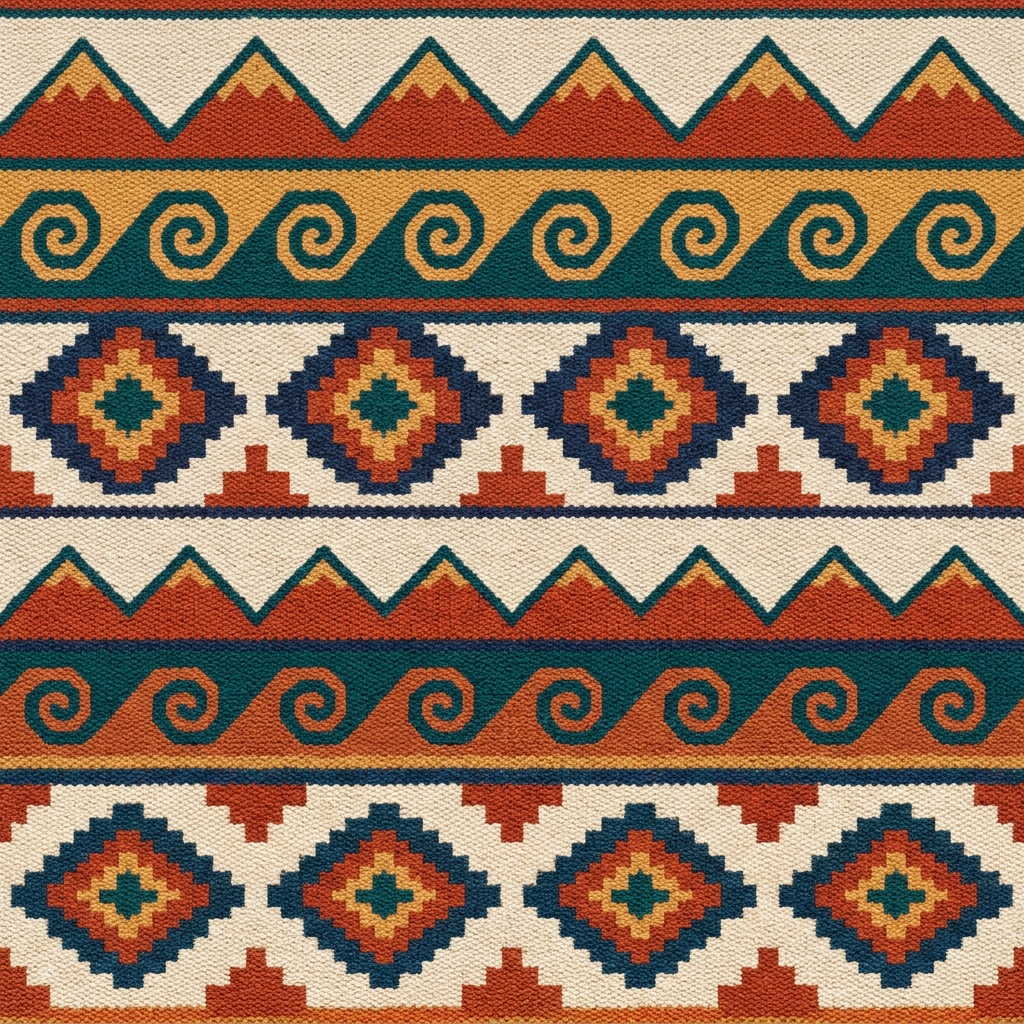
\includegraphics[width=0.40\textwidth]{assets/andean_textile.jpg}\par
\vspace{4pt}
\raggedright\fontsize{9}{11}\selectfont\textit{Nota.} Textura continua (\texttt{public/textures/andean\_textile.jpg}) con motivos geométricos de montaña y agua utilizada en la Estación 6.
\end{figure}

\subsection{Mecanismos de Accesibilidad Universal Implementados}

Siguiendo las recomendaciones de operabilidad y perceptibilidad de las pautas WCAG 2.2 (W3C, 2023), la interfaz superpuesta (\textit{HUD}) evita exigir acciones complejas de ratón. Los usuarios pueden rotar la mirada mediante botones dedicados (\textit{Izquierda}, \textit{Centrar}, \textit{Derecha}), activar un \textit{Paseo guiado} sin manos, ocultar la tarjeta narrativa para disfrutar una vista despejada, conmutar entre perspectiva de silla de ruedas (1,15 m) y vista de pie (1,65 m), ampliar la escala tipográfica hasta un 135\,\%, activar el tema de alto contraste, suprimir animaciones mediante \textit{Reducir movimiento} y regular independientemente el volumen del bosque o la velocidad de la voz narradora.

\section{Despliegue, Control de Versiones y Validación Técnica}

El código completo del prototipo, sus recursos gráficos y la documentación del Laboratorio 1 se gestionaron mediante Git y se publicaron en un repositorio público en GitHub utilizando GitHub CLI (\texttt{AMVMesias/sendero-vivo-3d}, rama \texttt{main}), excluyendo artefactos generados (\texttt{node\_modules/} y \texttt{dist/}) mediante \texttt{.gitignore}. Posteriormente, el proyecto se enlazó y desplegó en producción mediante Vercel CLI (\texttt{museo-abierto-3d.vercel.app}), generando el paquete optimizado de producción con Vite (\texttt{vite build}) en entorno de compilación remoto.

En cuanto a la verificación técnica realizada, se comprobó localmente la compilación limpia sin errores mediante \texttt{npm run build} tras incorporar los shaders GLSL, las once texturas continuas, los cinco arquetipos arbóreos, el sotobosque con helechos y arbustos, y la iconografía SVG. Asimismo, la inspección visual automatizada en navegador confirmó cero errores de consola o compilación WebGL/GLSL en estaciones representativas (Mirador, Árboles Abuelos y Cascada Viva), verificando la ausencia de recortes celestes, el flujo hídrico animado y las transiciones multizona del suelo; junto con la disponibilidad pública en Vercel (\texttt{200 OK}). La validación experiencial directa con participantes reales del grupo vulnerable se proyecta como fase de pruebas de usabilidad en el Laboratorio 2.

\section{Conclusiones}

La selección delimitada de personas con movilidad reducida y adultos mayores permitió diseñar un prototipo inmersivo donde la accesibilidad no constituye un añadido superficial, sino el eje estructural de la experiencia: desde la pasarela continua de 250 metros sin escalones hasta la cámara ajustable a 1,15 metros de altura y los controles libres de fatiga motriz. La integración del enfoque de interculturalidad crítica garantizó que el territorio y los oficios rurales se presenten a través de voces comunitarias dignas, articulando naturaleza, salud ancestral, gestión del agua y economía solidaria. Finalmente, la incorporación de texturas continuas con relieve, iconografía SVG personalizada, audio ambiental procedural y despliegue público en GitHub y Vercel demuestra la viabilidad técnica de construir soluciones inmersivas inclusivas accesibles desde cualquier navegador web sin barreras de hardware.

\newpage

% ============================================================================
% REFERENCIAS (NORMAS APA 7.ª EDICIÓN)
% ============================================================================
\section{Referencias}

\begingroup
\setlength{\parindent}{0pt}
\setlength{\parskip}{6pt}
\everypar{\hangindent=1.27cm \hangafter=1}

Asamblea Nacional del Ecuador. (2012). \textit{Ley Orgánica de Discapacidades} (Suplemento del Registro Oficial N.\textsuperscript{o} 796, 25 de septiembre de 2012).

Organización Mundial de la Salud. (2022). \textit{Informe mundial sobre la equidad en salud para las personas con discapacidad}. Organización Mundial de la Salud.

Organización Mundial del Turismo. (2014). \textit{Manual sobre turismo accesible para todos: Principios, herramientas y buenas prácticas. Módulo I: Turismo accesible -- Definición y contexto}. Organización Mundial del Turismo; Fundación ONCE; Red Europea de Turismo Accesible.

Walsh, C. (2009). \textit{Interculturalidad, Estado, sociedad: Luchas (de)coloniales de nuestra época}. Universidad Andina Simón Bolívar; Ediciones Abya-Yala.

World Wide Web Consortium. (2023). \textit{Web Content Accessibility Guidelines (WCAG) 2.2}. \\ \url{https://www.w3.org/TR/WCAG22/}

\endgroup

\end{document}
